\documentclass[utf8]{../IncArticle}
\graphicspath{{../}}
%\usepackage{color}
%\usepackage{todonotes}
% \usepackage{lmodern}
\usepackage{xcolor}

\colorlet{pcolor}{blue}
\colorlet{fcolor}{red}
\newcommand{\e}[2][fcolor]{\textcolor{pcolor}{[}\textcolor{#1}{#2}\textcolor{pcolor}{]}}





% *** PDF, URL AND HYPERLINK PACKAGES ***
%
\usepackage{url}

\title{Интерактивная методика извлечения семантической разметки
  текстовых документов, основанная на полисистеме онтологий
  \e{Первоначальный заголовок: Методика ПРИОБРЕТЕНИЯ знаний из
    текстовых документов, основанная на анализе ответов пользователя и
    полисистемы онтологий} }

% \AddAuthor{Черкашин}{Е}{вгений}{А}{лександрович}{Институт динамики систем и теории управления СО РАН, Иркутск, ул. Лермонтова 134, 664033}
% \AddAuthor{Черкашин}{А}{лександр}{К}{онстантинович}{Институт географии им. В.Б. Сочавы СО РАН, Иркутск, ул. Улан-Баторская 1, 664033}
% \AddAuthor{Бычков}{И}{горь}{В}{ячеславович}{Институт динамики систем и теории управления СО РАН, Иркутск, ул. Лермонтова 134, 664033}
% \AddAuthor{Паскал}{К}{ристина}{К}{онстантиновна}{Национальный исследовательский Иркутский государственный технический университет, Иркутск, ул. Лермонтова 83, 664074}
% \AddAuthor{Белых}{П}{олина}{В}{асильевна}{Институт динамики систем и теории управления СО РАН, Иркутск, ул. Лермонтова 134, 664033}

\AddAuthor{Черкашин}{Е}{вгений}{А}{лександрович}{}
\AddAuthor{Черкашин}{А}{лександр}{К}{онстантинович}{}
\AddAuthor{Бычков}{И}{горь}{В}{ячеславович}{}
\AddAuthor{Паскал}{К}{ристина}{К}{онстантиновна}{}
\AddAuthor{Белых}{П}{олина}{В}{асильевна}{}

\setcounter{page}{1}
\date{}
\begin{document}

\begin{abstract}
%\boldmath

  В докладе представляется идея подхода к представлению и индукции
  логического слоя представления содержимого, например, сайтов,
  юридических документов и т.п. Этот слой порождается на основе
  анализа результатов редактирования содержимого (контента) --- как
  текстовой составляющей, так и его существующей логической структуры.
  Варианты интерпретации того или иного изменения содержимого
  (исправление ошибки/значения или формирование нового высказывания)
  уточняются при помощи диалога с пользователем.  На принятие решения
  также влияют результаты анализа поведения пользователя, например,
  выделяются повторяющиеся переходы между редактируемыми документами
  определенных классов.

  Теоретической основой методики является представление предметной
  области в виде полисистемы онтологий, т.е. многослойной структуры
  понятий и отношений, которые отображаются между слоями через
  интерпретацию.  Полисистема онтологий, представленных в виде
  семантических сетей, позволяет организовать диалог с пользователем,
  упорядочивать и классифицировать факты о предметной области, а также
  получать новые интерпретации формируемых концептов.

  В качестве тестовой среды для разрабатываемых технологий выбрана
  автоматизация деятельности нотариальной конторы и документооборот
  административных, хозяйственных и научных подразделений бюджетного
  учреждения.  Документы, используемые в этих видах деятельности,
  обладают одним важным свойством --- содержащаяся в них информация
  представляется как в структурируемом, так и в неструктурируемом
  виде.

\end{abstract}

\begin{abstract}[english]
  \e[blue]{Here we have English abstract}
\end{abstract}


\introduction{}

В 2001 году Т.-Б.Ли предложил план развития интернет"=технологий
(семантический веб), который направлен на реализацию сетевых сервисов
со значительным уровнем интеграции логического слоя представляемой
информации.  Информация размечается семантически, а программные агенты,
используя эту информацию, производят ее обработку с целью решения
конкретных практических задач пользователя.

Одной из основных проблем семантического веба является тот факт, что
большинство пользователей решают свои практические задачи и не
заинтересованы повышении своей квалификации до уровня позволяющего
использовать эти технологии в полной мере.  В такой ситуации
технологические аспекты семантического веба должны быть полностью
скрыты, а программное обеспечение должно "варить кашу из
топора".  Необходимо разрабатывать программное обеспечения управления
содержимым сайтов и юридических документов как технологий приобретения
знаний, где пользователю предоставляется роль источника дополнительной
информации для интегрированного в систему механизма поддержки принятия
решений.

Идею подхода удобно излагать на примере юридических документов,
которые в большинстве случаев содержат сведения об отношениях между
физическими и юридическими лицами, а также другими элементами.  Эти
сведения в исходной или преобразованной форме используются в других
документах.  Поэтому имеет смысл для каждого документа извлекать и
хранить достаточно детально представленное логическое описание таких
сведений, которое преобразуется в текстовый документ при помощи
шаблонов.  Вариант преобразования определяется отображаемым документом,
т.е. документ задает контекст представления логического слоя.

К настоящему времени технологии Семантического Веба (СВ) предоставляют
формальные механизмы представления указанных отношений при помощи
стандартных форматов и структур данных, а также несколько механизмов
их логической обработки.  Логический слой представления информации в СВ
представляет собой граф, состоящий из концептов (понятий) и отношений
между ними.  В частности в юридическом документе физические и
юридические лица находятся с этим документом в отношении
``часть--целое'', а также в их более точных и содержательных вариантах.

В настоящее время большинство вариантов использования онтологических
моделей предметных областей сводятся к решению задачи уточнения
диапазона релевантных документов в процессе поиска.  Автоматизация
извлечения онтологий из текстовых документов базируется на
сканировании хранилищ документов: содержимого текста документов и их
метаданных, анализ результатов сканирования.  Наблюдение за поведением
людей в процессе подготовки различных документов приводит к
заключению, что содержательные части документов, которые и
представляются в логическом слое, как правило, находятся в тех местах
текста, где чаще всего пользователи производят изменения.  Поэтому,
информационная система, автоматизирующая процессы подготовки
документов, должна отслеживать изменения, вводимые пользователем, во
времени и в пространстве версий.  Версии порождаются копированием
документа или использование его в виде шаблона нового
документа.  Подвергаться анализу должна вся совокупность
изменений.  Предлагаемый подход позволяет сузить объем обрабатываемой
информации за счет фокусировки алгоритмов анализа данных вблизи
изменений.  Границы изменений задаются, например, свойствами формата
представления текста документа (гипертекстовой разметкой) или
существующей логической структурой одной из его \e{документа} версий.

Элементы логического слоя (концепты, объекты и отношения между ними)
формируются в результате применения алгоритмов анализа данных и
интервьюирования пользователя.  Среда, контекст, \e{приобретения знаний}
включает в себя:
\begin{itemize}
\item полисистему онтологий, совокупно описывающую предметные области,
  имеющие отношение к представлению документа как структуры данных,
  так и его содержательного смысла;
\item история изменения документа и его логического слоя;
\item список последних изменений в текущей транзакции (новой версии);
\item история действий пользователя в системе (пользователь, например,
  выполняет типичный набор действий по подготовке стандартного пакета документов);
\item ответы пользователя на утоняющие вопросы системы, цель которых
  --- определить \e{истинные намерения пользователя} смысл сделанных исправлений.
\end{itemize}

В результате анализа этих данных формируются новый набор троек вида
\texttt{<subject, relation, object>}, \e{представляющих новые данные
нового документа/версии, представленные в логическом
слое}.  Накопленные логические слои документов необходимо периодически
также сканировать на выявление стойких функциональных зависимостей
между значениями объектов.  В результате этого анализа, предлагается
совершенствовать формат представления данных слоя, например применяя
реляционные таблицы в качестве хранилищ.  \e{Метод функциональных
зависимостей применяется наоборот (т.е. данные - анализ - структура)}.

Сеть взаимодействующих программных систем, в которых реализованы
перечисленные функции, обладает многими свойствами социальной сети.
Основными видами обработки информации в такой сети являются ввод,
хранение, фильтрация и передача, т.е. интеграция данных, а не их
агрегация с целью порождения комплексных отчетов.  Поэтому применения
специальных методологий проектирования программного обеспечения при
разработке таких систем (или подсистем приобретения знаний
описываемого вида), например, объектно"=ориентированных технологий, не
является значительным преимуществом.  Гораздо важнее обеспечить
возможность функционирования программ в доступной недорогой серверной
среде (хостинге) и создания каналов данных на основе современных
стандартных форматах данных и сетевых интерфейсов прикладного
программирования.  Обработку информации агрегированного типа в
социальных сетях выполняют, преимущественно, пользователи и, как
правило, подсознательно.

Интересным свойством такой социальной сети, реализующей, фактически,
распределенный документооборот, является требования к организации
обмена данными между пользователями в процессе подготовки документов
преимущественно в режиме off-line.  Современные информационные
технологии позволяют хранить данные логического слоя в разметке
электронных документов \ref{microformats,RDFa} и в виде QR-кодов,
сопровождающих печатные варианты документов.

В качестве платформы для тестирования разрабатываемых технологий
выбрана автоматизация деятельности российского нотариального
офиса.  Операции, выполняемые над документами и шаблонами представимы
как изменения содержания текста документа и его логического
слоя.  Примерами таких операций выступают копирование логического слоя
из одного документа в другой, смена ролей лиц в документа в процессе
его подготовки, накапливание базы данных клиентов и другой справочной
информации, \e{доступ к которой организуется при помощи быстрого
контекстного поиска}. \e[green]{Далее содержимое сайтов и документов будем
просто называть просто ``документ''}.

\section{Представление логического и презентационного слоя документа}

Стандартный формат представления знаний RDF описывает информационные
ресурсы при помощи троек вида \texttt{<subject, relation, object>} в
некотором контексте.  Множество всех троек задают некоторый граф (сеть)
объектов и концептов, а также отношений между ними, формируя систему
знаний предметной области.  Такое описание предметных областей удобно
разбивать на подграфы, организовывать их в иерархические комплексы
\cite{b4}, порождая иерархии контекстов.  В общем случае, контекст
влияет на способ или вариант интерпретации троек.  Например, фамилия и
данные паспорта в нотариальных документах могут располагаться в разных
частях текста, однако относятся к одному контексту --- личным данным
пользователя.  \e{Ну и что за странный пример??}

Механизм порождения текстов документов на основе данных логического
слоя и шаблонам представления рассмотрен нами в [-2-].  В предлагаемом
подходе шаблоны для отображения логического слоя документа также
хранятся в графе.  \e[green]{Включить все оттуда, т.к. в русскоязычной
  литературе не печатано.  }\e{We also represent the views and
  algorithms implementing controllers in the sense of MVC (Model View
  Controller) technique with triples \cite{b5}}.


Содержимое документа в общем случае представляется в виде дерева, где
большинство узлов являются и субъектами и объектами
одновременно. Исключения составляют корневой узел (он является только
субъектом) и листовые узлы (только объекты).  В иерархии документов
корневые узлы связаны \e{другими} отношениями, например, организацией
документов в тематические иерархии и кластеры.

\e[cyan]{включить Chameleon надо не позже этого места ;-)}

Одним из основных моментов исследования --- это разработка методики
адаптации процесса извлечения разметки к процессу редактирования
документа.  Далее будем предполагать, что изменение, вносимое
пользователем, влияет на содержательный смысл текста документа
(изменяемой структуры), соответственно изменяя его логический слой.
Т.е. мы далее не рассматриваем простое исправление ошибки, которое
представляет собой изменение значения поля \texttt{object} и только
его в тройке, или исправление текста абзаца, в том числе в исходном
шаблоне.  Содержательное изменение в основном приводит к формированию
новой тройки между каким-либо субъектом в контексте документа и
изменяемым значением.  Анализ изменений в тексте документа направлен
на формирование таких новых данных и знаний, при этом система играет
активную роль, а пользователь является источником дополнительной
информации.

Обогащение семантической разметки в среде, содержащей логическую
структуру исходного документа, которая уже храниться в базе данных.  И
тогда перечень данных, используемых системой для принятия решения
включает\,:
\begin{enumerate}
\item исходную версию документа;
\item изменения текста документа, представленные в виде стандартного
  diff-формата \cite{b9};
\item ответы пользователя на вопросы, задаваемые системой; ответы
  уточняют смысл изменений (\e{что имел ввиду пользователь});
\item перечень действий пользователя, предшествовавших данному
  исправлению документа. \label{em:behav}
\end{enumerate}
Суть п.~\ref{em:behav}, например, проявляется при создании нового
документа из шаблона или его копии, что вообще говоря, приводит к
необходимости заполнения определенного перечня полей \texttt{object}
уже существующих троек.  Таким набором, например, выступает
стандартный набор полей для идентификации физического лица (ф.и.о.,
данные паспорта, адрес места жительства и т.п.) в нотариальной
доверенности.

Если же документ модифицирован частично, то данное изменение
интерпретируется как (\e{если это не простое исправление ошибки}) \e{a refinement of the logical structure of subject, extraction of a relation and an object; this corresponds to a new triple connecting the subject to the new object (changed value); the user must choose the \e[blue]{subject} of the new triple.}

Новый субъект должен быть выбран из списка (дерева) всех существующих
в контексте документа субъектов.  Далее для этого субъекта формируется
список всех возможных отношений, который формируется из всех возможных
отношений для этого субъекта и его класса, включая классы-предки.
Пользователю необходимо выбрать одно отношение для формируемой тройки.
\e{Надо где-то сказать про то, как сужать данный список.}  Если в
списке не содержится необходимого отношения, то его необходимо
определить.  \e{Что-то про определение...}  Новое отношение является
всегда \e{уточняющим} подклассом какого-либо существующего в списке
отношения.  Чтобы не \e{загрязнять} систему новыми сущностями\e{,
обозначающими отношения,} сформированными неопытными и невнимательными
пользователями, необходимо периодически проводить анализ этих
отношений инженерами знаний.  Их задача исключить дублирующие (эквивалентные),
противоречивые и семантически неточные отношения, и производить
реорганизацию (refactoring) онтологической модели.

Если объект какой-либо тройки удален, то и вся тройка должна быть
также удалена из логического представления документа.  Процесс
удаления должен контролироваться анализом минимальной структурной и
семантической непротиворечивости.  Например, при удалении из
доверенности физического лица, должны быть удалены и его паспортные
данные (\e{другое дело - имеет ли смысл удалять физ.лицо из
  доверенности.}). В результате анализа либо удаление разрешается,
либо запрещается, либо создает цепочку удалений троек, как в примере с
физическим лицом.  Для реализации этой функции каждый класс субъектов
необходимо сопроводить перечнем троек, которые необходимы для
формирования его содержательного базиса.

Добавление троек, в общем случае, приводит к добавлению новых
субъектов и отношений.  Примером такой ситуации выступает создание
трехстороннего договора из двустороннего добавлением нового физического
лица.  При этом также необходимо, в общем случае, заполнить
необходимые поля паспортных данных, а также установить отношения между
контекстом, субъектами документа и новым физическим лицом.

\section{Теоретическое обобщение процесса извлечения разметки}

Вышеописанный процесс является пошаговой реализацией процедуры
полисистемного анализа и синтеза \cite{father} (ППАС), которая
является общей процедурой системного анализа предметных областей.
Суть процедуры состоит в том, что предметная область и все ее объекты
и процессы расслаиваются по солям и представляются концептами и
отношениями (морфизмами) в многомерном пространстве слоев-координат.
В отличие от классического системного подхода, где принцип
взаимодействия элементов является фундаментальным, полисистемный
анализ предполагает выполнение гипотезы расслоения, т.е. он
предполагает, что объект исследования представим в виде
заимонепересекающихся слоев (подмножеств в частном случае),
подобластей. \e{Что там с концептами, отношениями, морфизмами интерпретациями??}  Таким образом, полисистема и является системой сама по
себе с более общей точки зрения, а ППАС --- это новый вид системного
анализа.

В общем виде приложение ППАС к задаче автоматизации построения
разметки документов состоит в построении многослойной декомпозиции
предметной области и данных документа. В качестве слоев выступают
различные аспекты представления документа\,: структурная
(мереологическая) организация документа, концептуальное моделирование
предметной области документа, наследование свойств документов,
моделирование отношений между физическими и юридическими лицами,
модели документов в \e{дионическом представлении} и т.п.

В соответствии с ППАС \cite{father} каждому концепту одного слоя
полисистемного расслоения должен соответствовать (через интерпретацию)
концепт во всех других слоях, а также отношения с другими концептами в
его слое.  В идеальном случае в каждом слое в результате выполнения
процедуры должна быть построена законченная теория.  Все теории
\e{отличается своими фундаментальными основаниями}, но также являются
схожими через интерпретацию (подстановку, замену) концептов.  Все это
позволяет нам индуцировать (порождать) новые аксиоматические теории
предметных областей по образу и подобию уже построенных.  Каждый
системный уровень (слой) знаний также многократно и последовательно расслаивается,
порождая полисистемное представление исследуемого объекта.  Таким
образом, все системные теории комбинируются в объединенную модель,
описывающую и предметную область и объект исследования.  \e{в нашем
  случае --- документ.}

В нашем случае ППАС направлена на порождение (формирование) троек и
контекстов (слоев).  Получаемые классы документов, физических и
юридических лиц и других объектов формируют множество концептов
теории соответствующего слоя.  Выделяя новый класс или отношение между
классами, необходимо \e{обязательно} установить связь с концептами и отношениями в
других слоях (интерпретацию).  Для удобства восприятия необходимо
также создавать для получаемых концептов определения на естественном
языке, соответствующее слою.

Each of new concept (a class) as we described in the previous section
is to be inherited from a parent class, thus, it can be interpreted in
other ontologies as either a concept that corresponds to the parent
class or to a new inherited class.  This case the user interview also
organized to obtain a description of the class and the relation.

Использование ППАС позволяет нам \e{справиться с} полнотой понятий и отношений
порождаемого слоя (\e{описания и его теории}) (\e{как это в диссертации Ковалева}
\ldots{} \cite{sergey}), а также непротиворечивости (при помощи
верификации онтологии).

\subsection{Ведение диалога с пользователем}

\e{... на базе полисистемы онтологий.}

Как было сказано выше, любая моделируемая предметная область \e{может
  быть} декомпозирована в полисистему понятий, объектов и отношений. С
общей точки зрения полисистема --- иерархическая структура,
составленная из непересекающихся слоев.  Каждый уровень включает
систему концептов, объектов и отношений между ними.  In a fibrated polysystem, concepts belonging to a layer are morfed (mapped) into concepts in other layers via concept interpretation of one layer (projection, theory, science, domain) into concepts of other layer.  All the concepts are interpreted by concepts of the abstract system layer.  The interpretation feature of polysystem layers could be used to drive user interview dialog on the base of an inference by analogy represented as movement along relations and morphs in the polysystem of ontologies.

Consider simple family relationships in fig.~\ref{OPSA}, where most of the obvious relations are hidden to make the figure more readable.  There are four main layers in the figure, which model corresponding aspects of Bob's family: layer 1 represents the family itself, it is the only layer having a-box entities; layer 2 represent main roles of individuals in a family; layer 3 shows genders as two opposites; and later 4 corresponds to mereological metomodel ``whole--parts''.

Let's construct a list of questions to determine a role of Jul in Bob's family.  It is supposed we know only that Jul is a female.  To put Jul in layer 1, we must ask a general question: ``Is Jul a part of Bob's family?'' The question is constructed according to a following intuitive inference.  All relations between a family and its members are kinds of ``partOf:'' relation from layer 4.  This fact is shown as an arrow, which denote a contravariant functor from category of Layer 2 to category of Layer 4, from relation hasFather: of Layer 2 to ``partOf:'' of Layer 4, other four arrows are hidden.  So, in order to determine the fact that Jul is a member of Bob's family, it is sufficient to ask ``Is Jul partOf: Bob's-family?''.  The identifier of the example family is devised from the tradition to name families after their master of housekeeping (MOH) person, that is denoted by arrow from individual Bob (layer 1) to concept MOH (layer 2).

If user answered positively (Jul is a part of the family), then we must refine her role, as partOf: is not a role allowed to be used in layer 1.  Jul is a female (by definition), so she cannot be father and son.  If she is, she must be male, but it is not as male and female are formally opposite concepts.  If multiplicity of relations in the layer are defined, then we will also know, that the family already has mother.  The only possible choice is Jul is daughter, resulting an another general question:''Is Jul daughter?'' If the answer to the second question is also positive, finally a new triple constructed <Bob's-family hasDaughter: Jul>.

If, e.g., gender of Jul is unknown, then the second question is constructed as a special question ``What role has Jul in Bob's family?'' and a list of two possible answers is shown: ``hasDaughter:'' and ``hasSon:''.  Or it can be constructed as an alternative question ``Is Jul plays hasDaughter: or hasSon: role in the family?'', but in this case the sentence is more weird with respect to English.

\begin{figure}
\centering\sf
\def\svgwidth{0.9\linewidth}
\input{layer.pdf_tex}
\caption{An  Usage Example of an Ontology Polysystem}
\label{OPSA}
\end{figure}



(HERE: a generalizing resume paragraph needed.  )

(About polysystem of ontologies).

(procedure of fibration)

(procedure of completeness reconstruction): (About mapping via functors).

(Induction of notions, suppositions of fibrations).

(wikipedia and Google search systems).

(!! Systems of complexes. !!)

\section{An Office Usage of the Technique}

One of the applications of the technology under development is document preparation automation of a notary office.  Notary office in Russia generate vast amount of printed documents.  The documents contain both formalized and unformalized data in a balance reasonable for our study.  For example, formalized data are the passport data of individuals, registration data of vehicles.  Data of this kind are passed from one document to other documents mostly sturcturized and unchanged, raising a bindles of related documents.  The document content structure significantly depends on entry fields’ data filled in: form of notary signature field depends on legal capacities of the individuals mentioned in the main document body.  At present templates of the documents are prepared by a programming engineer collaborating with a professional secretary and verified by supervising notary.  Unformalized data are various enumerations of legal empowerments of the individuals, article codes, and explanatory text.

Application of the semantic approach to the logical layer representation of the notary document content is aimed at involvement of the secretaries (people with low engineering skills) into the processes of the document instances preparation from the existing templates and into the development of the templates and constructing their hierarchical arrangement.

Logical layer of a notary document consists of hierarchy of subjects.  The subjects relate to each other on various abstraction levels, e.g., in a letter of attorney there are at least two individuals, the first one is principal, and the second one is trusted (proxy).  For each individual passport, data and place of residence are defined.  The letter can contain other person data, e.g., for partially capable children.  All the individuals are in explicit relation to the document.  The triples <letatt998 containsPrincipal indiv\_78> and <letatt998 containsProxy indiv\_79> could define a principal and proxy to the document.  The mentioned relations are specifications of abstract hasIndividual and structuralElement relations.  This multilevel approach allows us visually represent hierarchical structures of the document, having interpreted the relations as structural elements, and in the same time to associate individuals with other roles in new documents, swap roles during editing.  The swap function is implemented as user interface widget, which recognizes certain subject-to-subject relation patterns in the document body and interprets semantics of the relations as possible action.  A general graph structure of the abstract level of a notary office automation ontology is drawn in fig.~\ref{notaryontology}.

[The flexibility and minimum resources and administration requirements criteria are of very importance to choosing database providing information resources storage as triples.  The database management systems as DB2, Oracle and SQL Server cannot fulfill requirements because after running the operation is performed as a separate process.  Also application and DBMS interaction should be implemented through interprocess communication form.

Solution to these problems is achieved by using the built-in database management systems that provide communication with the application at the same level of address space.  This allows the application based on the built-in database to be efficient and autonomous.

Kyoto Cabinet is a library of routines for managing a database.  The database is a simple data file containing records, each is a pair of a key and a value.  Every key and value is serial bytes with variable length.  Both binary data and character string can be used as a key and a value.  Each key must be unique within a database.  There is neither concept of data tables nor data types.  Records are organized in hash table or B+ tree.  \cite{b1}

Availability of funds to work with triplets described in the standard RDF is an advantage database management system Kyoto Cabinet over other embedded systems is.  In this case the developer does not need to spend time on design and implementation of the data model so that its performance on this task is increased.

1.	Kyoto Cabinet. URL: http://fallabs.com/kyotocabinet/ (дата обращения: 20.02.2014).]

\begin{figure}[!t]
\centering
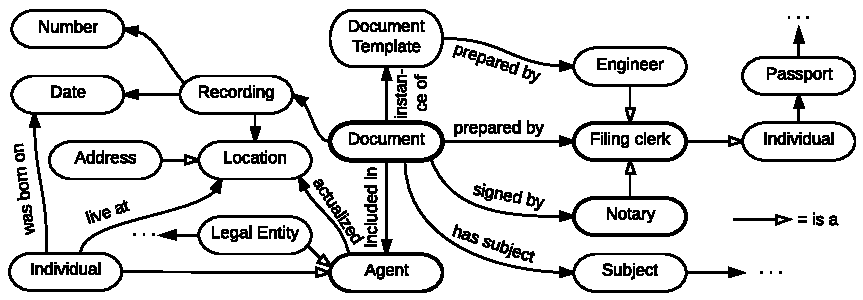
\includegraphics[width=\linewidth]{DocumentOntology-en.pdf}
% where an .eps filename suffix will be assumed under latex,
% and a .pdf suffix will be assumed for pdflatex; or what has been declared
% via \DeclareGraphicsExtensions.
\caption{An upper layer of notary office ontology}
\label{notaryontology}
\end{figure}


\conclusion
An approach to representation of logical layer of a document based on RDF (Resource Description Framework) is proposed.  The approach allows us to formalize the structure and semantic relation of the document, and also store data to render the document as HTML-page in the same data format - RDF.  XML and RDF allow us to join logical and presentation aspects of the document within the same storage engine.  The engine stores data as an onology, i.  e., set of triples <subject, relation, object>.  A technique for HTML-rendering from the logical layer is described.  The resulting document will contain the logical layer as a RDFa markup.  The generated RDFa-markup is used at client side by web-browser for control of WYSIWYG-editing of the document.  Text elements are modified with special widgets appearing in the user interface on an mouse event.  A technique for organization of an interactive process of logical layer forming of the document content on the base of modifications analysis of the document content introduced by user.  An example of application of the technologies under development in a notary office is presented.  Thus, we shown that RDF format mixed with XML allows us to represent logical layer of meaningful information of a document, as well as sharing common data between documents.

On the base of the technology a network of document data exchange can be devised.  The security of the document transmission can be provided as off-line data streams: each physical document is accompanied with its bar- or QR-code encoding the corresponding RDF-data of the transferred document.  This can result in a semantic network analogous to nowadays social networks.

A part of the paper devoted to consideration of organizational problems, such as involving knowledge engineers in a refinement process of generated parts of the ontologies; partial automatic ontology verification; implementing secure ways of personal data transfer and processing.  The properties of the document exchange network will be similar to social networks, and, probably, can be further developed and investigated the same way.



% use section* for acknowledgement
\thanks Результаты исследований получены при поддержке Интеграционного
междисциплинарного проекта СО РАН №17 «Создание сервисов и
инфраструктуры научных пространственных данных для поддержки
комплексных междисциплинарных научных исследований Байкальской
природной территории».

\begin{thebibliography}{11}
\bibitem{TBL2001} T. Berners-Lee, J. Hendler and O. Lissila. \emph{The Semantic Web A new form of Web content that is meaningful to computers will unleash a revolution of new possibilities.}\hskip 1em plus 0.5em minus 0.4em\relax  Scientific American, May 17, 2001, pp.1-18. URL: http://sciam.com/article.cfm?articleID=00048144-10D2-1C70-84A9809EC588EF21. (access date: 05.09.2013).
\bibitem{q1}
Social network - Wikipedia, the free encyclopedia. URL: \url{http://en.wikipedia.org/wiki/Social_network} (access date: 20.08.2013).
\bibitem{q2}
Chameleon – Chameleon 2.10 documentation. \url{http://chameleon.readthedocs.org/en/latest/} (access date:  20.08.2013).
\bibitem{q3}
Virtuoso Open-Source Edition URL: \url{http://virtuoso.openlinksw.com/dataspace/doc/dav/wiki/Main/} (access date: 30.05.2013).
\bibitem{q4}
PIZZA Protege OWL tutorial at Manchester (School of Computer Science - The University of Manchester)  URL:\url{http://owl.cs.manchester.ac.uk/tutorials/protegeowltutorial/} (access date: 20.09.2013).
\bibitem{q5}
SWI-Prolog's home. URL: \url{http://www.swi-prolog.org/} (access date: 20.08.2013).
\bibitem{q6}
The Protégé Ontology Editor and Knowledge Acquisition System. URL: \url{http://protege.stanford.edu/} (access date: 20.08.2013).
Semantic MediaWiki. URL: \url{http://semantic-mediawiki.org/} (access date: 20.08.2013).
\bibitem{q7}
N.Heino, S.Tramp, N.Heino, S.Auer. Managing Web Content using Linked Data Principles – Combining semantic structure with dynamic content syndication. Computer Software and Applications Conference (COMPSAC), 2011 IEEE 35th Annual. pp. 245 - 250. URL:\url{http://svn.aksw.org/papers/2011/COMPSAC_lod2.eu/public.pdf} (access date: 30.05.2013).
\bibitem{q8}
Cherkashin E.A., Paramonov V.V., et al, Model Driven Architecture is a Complex System, E-Society Journal Research and Applications. Volume 2, Number 2, 2011, pp. 15-23.
\bibitem{q9}
Father

% Format examples.
\bibitem{m1} Автор И.О. Название книги --- М.: Издательство, 2002. --- 700~с.
\bibitem{m2} Автор И.О. Статья // В книге --- Ижевск: Издательство, 2011. --- С.~71-90.
\bibitem{m3} Сайт ТИПД-2014 // \url{http://itpa2014.conf.udsu.ru/}
\end{thebibliography}

% that's all folks
\end{document}

%% Local Variables:
%% eval: (ispell-change-dictionary "ru_RU_hunspell")
%% TeX-master: t
%% TeX-PDF-mode: 1
%% TeX-source-correlate-mode: 1
%% TeX-source-correlate-start-server: nil
%% End:
